\documentclass[12pt, a4paper]{article}

\usepackage[utf8]{inputenc}
\usepackage[T5]{fontenc}
\usepackage[vietnamese]{babel}
\usepackage{amsmath}       
\usepackage{geometry}        
\usepackage{tikz}          
\usetikzlibrary{calc}     
\usepackage{graphicx}      
\usepackage{float}

\geometry{
    a4paper,
    total={170mm,257mm},
    left=30mm,
    right=20mm,
    top=20mm,
    bottom=20mm,
}

\begin{document}
\begin{titlepage}
    \begin{tikzpicture}[remember picture, overlay]
        \draw[color=cyan!70!blue, line width = 2pt] 
            ($(current page.north west) + (2cm,-1.5cm)$) 
            rectangle 
            ($(current page.south east) + (-1.5cm,1.5cm)$);
        \draw[color=cyan!70!blue, line width = 0.5pt] 
            ($(current page.north west) + (2.1cm,-1.6cm)$) 
            rectangle 
            ($(current page.south east) + (-1.6cm,1.6cm)$);
    \end{tikzpicture}

    \begin{center}
        \vspace*{0.8cm}
        \textbf{\large BỘ GIÁO DỤC VÀ ĐÀO TẠO} \\[0.2cm]
        \textbf{\Large TRƯỜNG ĐẠI HỌC SÀI GÒN} \\[0.2cm]
        \textbf{\large KHOA TOÁN - ỨNG DỤNG} \\[2.5cm]

        
\includegraphics[width=4cm]{logo.png} \\[2cm] 
        
        \vspace{1.5cm}
        \textbf{\Large BÀI TẬP NHÓM GIỮA KỲ} \\[0.5cm]
        \textbf{\large Học phần: Thống kê nhiều chiều} \\[2cm]

        \begin{flushleft}
            \large
            \hspace{1.5cm} \textbf{Giảng viên hướng dẫn:} Lương Thị Hồng Cẩm \\[0.5cm]
            \hspace{1.5cm} \textbf{Sinh viên thực hiện:} \\[0.2cm]
            \hspace{2.5cm} 1. Nguyễn Trương Cao Sơn \hspace{0.5cm} MSSV: 3123580040 \\[0.2cm]
            \hspace{2.5cm} 2. Phan Đồng Minh Quân \hspace{0.75cm} MSSV: 3123580038 \\[0.2cm]
            \hspace{2.5cm} 3. Võ Minh Tiến \hspace{2.3cm} MSSV: 3123580053 \\[0.5cm]
        \end{flushleft}

        \vfill
        {\large TP Hồ Chí Minh, năm 2026}
        \vspace*{0.5cm}
    \end{center}
\end{titlepage}

\newpage

\section*{BÀI 1: Phân phối của vector biến đổi}

\textbf{1. Xác định ma trận biến đổi tuyến tính $A$}

Từ hệ thức $Y_1 = X_1 - X_2$ và $Y_2 = X_2 - X_3$, ta có $Y = AX$ với ma trận hằng số $A$ cấp $2 \times 3$:
\[ A = \begin{pmatrix} 1 & -1 & 0 \\ 0 & 1 & -1 \end{pmatrix} \]

\textbf{2. Vector kỳ vọng $\mu_Y$}

Áp dụng tính chất kỳ vọng của biến đổi tuyến tính, $\mu_Y = E[AX] = A\mu$:
\[ \mu_Y = \begin{pmatrix} 1 & -1 & 0 \\ 0 & 1 & -1 \end{pmatrix} \begin{pmatrix} \mu_1 \\ \mu_2 \\ \mu_3 \end{pmatrix} = \begin{pmatrix} \mu_1 - \mu_2 \\ \mu_2 - \mu_3 \end{pmatrix} \]

\textbf{3. Ma trận hiệp phương sai $\Sigma_Y$}

Áp dụng tính chất phương sai của biến đổi tuyến tính, $\Sigma_Y = \text{Var}(AX) = A\Sigma A^T$:
\[ \Sigma_Y = \begin{pmatrix} 1 & -1 & 0 \\ 0 & 1 & -1 \end{pmatrix} \begin{pmatrix} \sigma_{11} & \sigma_{12} & \sigma_{13} \\ \sigma_{12} & \sigma_{22} & \sigma_{23} \\ \sigma_{13} & \sigma_{23} & \sigma_{33} \end{pmatrix} \begin{pmatrix} 1 & 0 \\ -1 & 1 \\ 0 & -1 \end{pmatrix} \]
Khai triển phép nhân ma trận, ta được:
\begin{itemize}
    \item Phần tử $(1,1)$: $\sigma_{11} - 2\sigma_{12} + \sigma_{22}$
    \item Phần tử $(2,2)$: $\sigma_{22} - 2\sigma_{23} + \sigma_{33}$
    \item Phần tử $(1,2)$ và $(2,1)$: $\sigma_{12} - \sigma_{22} - \sigma_{13} + \sigma_{23}$
\end{itemize}
Suy ra:
\[ \Sigma_Y = \begin{pmatrix} \sigma_{11} + \sigma_{22} - 2\sigma_{12} & \sigma_{12} + \sigma_{23} - \sigma_{22} - \sigma_{13} \\ \sigma_{12} + \sigma_{23} - \sigma_{22} - \sigma_{13} & \sigma_{22} + \sigma_{33} - 2\sigma_{23} \end{pmatrix} \]

\textbf{Kết luận:} Vector $Y$ tuân theo phân phối chuẩn đa chiều cấp 2: $Y \sim N_2(\mu_Y, \Sigma_Y)$.


\section*{BÀI 2: Hàm mật độ điều kiện}

\textbf{1. Tính chất phân phối điều kiện}

Dựa trên tính chất của phân phối chuẩn đa biến, phân phối điều kiện của vector con $X_1$ khi biết $X_2 = x_2$ là một phân phối chuẩn đa biến cấp $q$:
\[ (X_1 | X_2 = x_2) \sim N_q(\mu_{1|2}, \Sigma_{11|2}) \]

\textbf{2. Xác định các tham số đặc trưng}

Áp dụng công thức phần bù Schur (Schur Complement), các tham số điều kiện được xác định như sau:
\begin{itemize}
    \item \textbf{Vector kỳ vọng điều kiện:}
    \[ \mu_{1|2} = E[X_1 | X_2 = x_2] = \mu_1 + \Sigma_{12}\Sigma_{22}^{-1}(x_2 - \mu_2) \]
    \item \textbf{Ma trận hiệp phương sai điều kiện:}
    \[ \Sigma_{11|2} = \text{Var}(X_1 | X_2 = x_2) = \Sigma_{11} - \Sigma_{12}\Sigma_{22}^{-1}\Sigma_{21} \]
\end{itemize}
\textit{Lưu ý:} Ma trận hiệp phương sai điều kiện $\Sigma_{11|2}$ độc lập với giá trị cụ thể của vector $x_2$.

\textbf{3. Hàm mật độ xác suất điều kiện}

Hàm mật độ xác suất của $X_1$ khi cho trước $X_2 = x_2$ được biểu diễn bởi:
\[ f(x_1 | x_2) = \frac{1}{(2\pi)^{q/2} |\Sigma_{11|2}|^{1/2}} \exp \left\{ -\frac{1}{2} (x_1 - \mu_{1|2})^T \Sigma_{11|2}^{-1} (x_1 - \mu_{1|2}) \right\} \]
Trong đó, $\mu_{1|2}$ và $\Sigma_{11|2}$ là các tham số đã được xác định ở mục 2.

\section*{BÀI 3: Phân tích dữ liệu điểm thi}

\subsection*{1. Tính toán mẫu}

Từ bảng dữ liệu với $n = 10$ và $p = 2$ ($X_1$: Toán, $X_2$: Vật lý), ta có:

\textbf{Vector trung bình mẫu:}
\[ \bar{x} = \begin{pmatrix} \frac{1}{10} \sum X_{1i} \\ \frac{1}{10} \sum X_{2i} \end{pmatrix} = \begin{pmatrix} 7 \\ 6 \end{pmatrix} \]

\textbf{Ma trận hiệp phương sai mẫu} $S$ với $S_{jk} = \frac{1}{n-1} \sum_{i=1}^n (X_{ji} - \bar{x}_j)(X_{ki} - \bar{x}_k)$:
\[ S = \frac{1}{9} \begin{pmatrix} 20 & -3 \\ -3 & 28 \end{pmatrix} = \begin{pmatrix} 20/9 & -1/3 \\ -1/3 & 28/9 \end{pmatrix} \]

\textbf{Trị riêng của $S$:} Xét phương trình đặc trưng $|S - \lambda I| = 0$:
\[ \left( \frac{20}{9} - \lambda \right) \left( \frac{28}{9} - \lambda \right) - \left( -\frac{1}{3} \right)^2 = 0 \]
\[ \Leftrightarrow \lambda^2 - \frac{48}{9}\lambda + \frac{551}{81} = 0 \]
Giải phương trình ta được hai trị riêng: 
\[ \lambda_1 = \frac{29}{9} \quad \text{và} \quad \lambda_2 = \frac{19}{9} \]

\subsection*{2. Ước lượng vùng tin cậy 95\%}

\textbf{Phương pháp Bonferroni:} \\
Với độ tin cậy 95\%, ta có $\alpha = 0.05$. Giá trị tới hạn tra bảng $t_{n-1}\left(\frac{\alpha}{2p}\right) = t_9(0.0125) = 2.685$.
\begin{itemize}
    \item Khoảng tin cậy cho $\mu_1$:
    \[ \bar{x}_1 \pm t_9(0.0125)\sqrt{\frac{S_{11}}{n}} = 7 \pm 2.685\sqrt{\frac{20}{90}} \approx 7 \pm 1.266 \Rightarrow \mu_1 \in [5.734, 8.266] \]
    \item Khoảng tin cậy cho $\mu_2$:
    \[ \bar{x}_2 \pm t_9(0.0125)\sqrt{\frac{S_{22}}{n}} = 6 \pm 2.685\sqrt{\frac{28}{90}} \approx 6 \pm 1.498 \Rightarrow \mu_2 \in [4.502, 7.498] \]
\end{itemize}

\textbf{Phương pháp Hotelling:} \\
Hệ số khoảng tin cậy đồng thời là $\sqrt{\frac{p(n-1)}{n-p} F_{p, n-p}(\alpha)} = \sqrt{\frac{18}{8} F_{2, 8}(0.05)}$. \\
Tra bảng $F_{2, 8}(0.05) = 4.46$, suy ra hệ số bằng $\sqrt{2.25 \times 4.46} \approx 3.168$.
\begin{itemize}
    \item Khoảng tin cậy cho $\mu_1$:
    \[ 7 \pm 3.168\sqrt{\frac{20}{90}} \approx 7 \pm 1.493 \Rightarrow \mu_1 \in [5.507, 8.493] \]
    \item Khoảng tin cậy cho $\mu_2$:
    \[ 6 \pm 3.168\sqrt{\frac{28}{90}} \approx 6 \pm 1.767 \Rightarrow \mu_2 \in [4.233, 7.767] \]
\end{itemize}

\subsection*{3. Kiểm định giả thuyết}

Giả thuyết $H_0 : \mu_0 = \begin{pmatrix} 7 \\ 6 \end{pmatrix}$. \\
Thống kê kiểm định Hotelling $T^2$:
\[ T^2 = n(\bar{x} - \mu_0)^T S^{-1} (\bar{x} - \mu_0) \]
Do vector trung bình mẫu $\bar{x}$ tính được đúng bằng $\mu_0$ nên $(\bar{x} - \mu_0) = \begin{pmatrix} 0 \\ 0 \end{pmatrix}$. \\
Từ đó suy ra $T^2 = 0$.

Miền bác bỏ: $T^2 > \frac{p(n-1)}{n-p} F_{p, n-p}(\alpha) = \frac{18}{8} \times 4.46 = 10.035$. \\
\textbf{Kết luận:} Vì $T^2 = 0 < 10.035$, ta chưa đủ cơ sở bác bỏ $H_0$.

\subsection*{4. Thực hành R: Vẽ đồ thị vùng tin cậy và kiểm tra tính chuẩn}

\textbf{Mã nguồn R:}
\begin{verbatim}
# Nhập dữ liệu
Toan <- c(5, 6, 7, 8, 9, 5, 6, 7, 8, 9)
VatLy <- c(4, 7, 6, 9, 4, 8, 5, 7, 4, 6)
data_diem <- data.frame(Toan, VatLy)

# --- A. Kiểm tra tính chuẩn đa chiều bằng Mardia's test ---
# Yêu cầu cài đặt package 'MVN'
# install.packages("MVN")
library(MVN)
mvn_test <- mvn(data = data_diem, mvnTest = "mardia")
print(mvn_test$multivariateNormality)

# --- B. Vẽ đồ thị so sánh hai vùng tin cậy ---
# Yêu cầu cài đặt package 'car'
# install.packages("car")
library(car)

# Vẽ Ellipse Hotelling 95%
confidenceEllipse(lm(cbind(Toan, VatLy) ~ 1), levels = 0.95,
                  main = "So sanh vung tin cay Hotelling va Bonferroni",
                  xlab = "Toan (X1)", ylab = "Vat Ly (X2)",
                  col = "red", lty = 1, lwd = 2)

# Vẽ hình chữ nhật Bonferroni 95% (tọa độ lấy từ câu 2)
rect(xleft = 5.734, ybottom = 4.502, xright = 8.266, ytop = 7.498,
     border = "blue", lty = 2, lwd = 2)

# Thêm chú thích
legend("topright",
       legend = c("Hotelling Ellipse (95%)",
                  "Bonferroni Rectangle (95%)"),
       col = c("red", "blue"), lty = c(1, 2), lwd = 2)
\end{verbatim}

\vspace{0.5cm}
\noindent\rule{\textwidth}{0.4pt}
\vspace{0.3cm}

\begin{figure}[H]
    \centering
    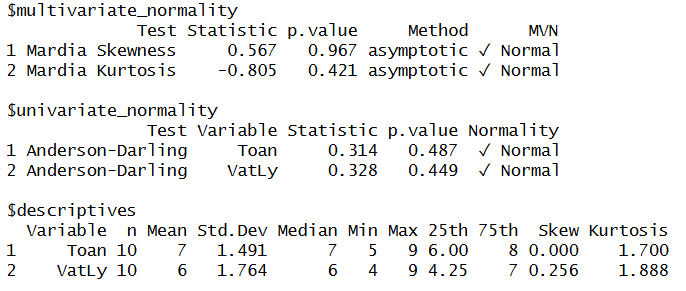
\includegraphics[width=0.9\textwidth]{kq_mardia_test.png}
    \caption{Kết quả kiểm tra tính chuẩn đa chiều (Mardia's Test) trên R}
\end{figure}

\begin{figure}[H]
    \centering
    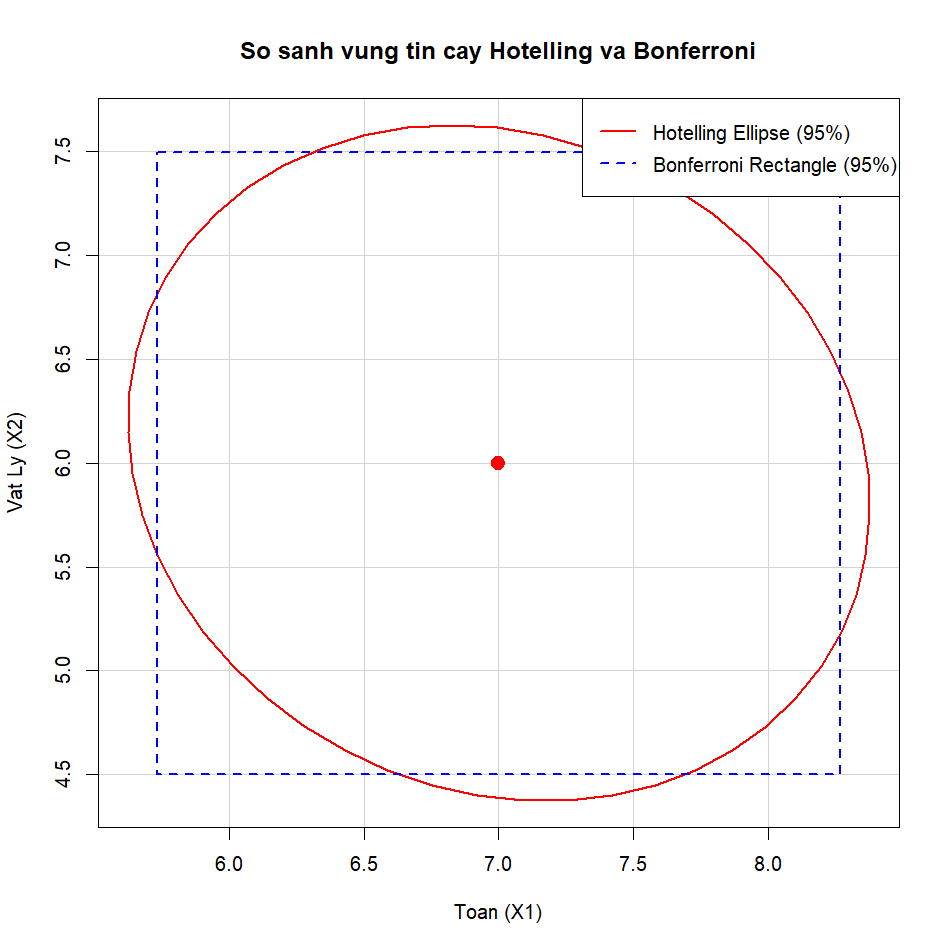
\includegraphics[width=0.8\textwidth]{Rplot.png}
    \caption{Đồ thị so sánh vùng tin cậy Hotelling và Bonferroni 95\%}
\end{figure}

% ==============================================

\textbf{b) Nhận xét kết quả chạy R}
\begin{itemize}
    \item \textbf{Về tính chuẩn đa chiều (Mardia's Test):} 
    Kết quả kiểm định Mardia cho thấy cả độ lệch (Mardia Skewness) với $p-value = 0.967$ và độ nhọn (Mardia Kurtosis) với $p-value = 0.421$ đều lớn hơn mức ý nghĩa $\alpha = 0.05$. R kết luận \texttt{Normal}, do đó ta có đủ cơ sở khẳng định dữ liệu điểm thi của 10 sinh viên tuân theo phân phối chuẩn đa chiều. Điều kiện để áp dụng thống kê Hotelling $T^2$ hoàn toàn được thỏa mãn.
    
    \item \textbf{Về đồ thị vùng tin cậy:} 
    Đồ thị hiển thị một hình Elip màu đỏ (Hotelling) nằm chéo theo chiều tương quan của dữ liệu và một hình chữ nhật viền xanh nét đứt (Bonferroni) bao bọc xung quanh. Hình Elip phản ánh được mối tương quan nghịch yếu giữa điểm Toán và Vật lý (hiệp phương sai $S_{12} = -1/3$), trong khi hình chữ nhật Bonferroni thì không xem xét hiệp phương sai này. Do đó, vùng Bonferroni bao phủ một diện tích rộng hơn nhưng kém chính xác hơn so với miền tin cậy đồng thời Hotelling.
\end{itemize}

\section*{BÀI 4: Phân tích phương sai nhiều chiều (MANOVA)}

\subsection*{A. Tính toán đặc trưng mẫu (Tính tay)}

\textbf{1. Các vector trung bình}

Dữ liệu gồm $g = 3$ nhóm, $p = 2$ biến. Tổng số quan sát $n = 12$. 
\\
Trung bình từng nhóm:
\[ \bar{x}_1 = \begin{pmatrix} 6 \\ 8 \end{pmatrix}, \quad \bar{x}_2 = \begin{pmatrix} 2 \\ 4 \end{pmatrix}, \quad \bar{x}_3 = \begin{pmatrix} 3 \\ 2 \end{pmatrix} \]

Vector trung bình chung toàn bộ dữ liệu:
\[ \bar{x} = \frac{n_1\bar{x}_1 + n_2\bar{x}_2 + n_3\bar{x}_3}{n} = \frac{5 \begin{pmatrix} 6 \\ 8 \end{pmatrix} + 3 \begin{pmatrix} 2 \\ 4 \end{pmatrix} + 4 \begin{pmatrix} 3 \\ 2 \end{pmatrix}}{12} = \begin{pmatrix} 4 \\ 5 \end{pmatrix} \]

\textbf{2. Ma trận tổng bình phương và tích chéo}

\begin{itemize}
    \item \textbf{Ma trận nội bộ nhóm} $W = W_1 + W_2 + W_3$:
    \\
    Tính trên từng nhóm theo công thức $\sum (x_{ij} - \bar{x}_i)(x_{ij} - \bar{x}_i)^T$, ta có:
    \[ W_1 = \begin{pmatrix} 10 & -6 \\ -6 & 8 \end{pmatrix}, \quad W_2 = \begin{pmatrix} 2 & -3 \\ -3 & 6 \end{pmatrix}, \quad W_3 = \begin{pmatrix} 6 & -4 \\ -4 & 4 \end{pmatrix} \]
    \[ \Rightarrow W = \begin{pmatrix} 18 & -13 \\ -13 & 18 \end{pmatrix} \]

    \item \textbf{Ma trận giữa các nhóm} $B = \sum n_i (\bar{x}_i - \bar{x})(\bar{x}_i - \bar{x})^T$:
    \[ B_1 = 5 \begin{pmatrix} 2 \\ 3 \end{pmatrix} \begin{pmatrix} 2 & 3 \end{pmatrix} = \begin{pmatrix} 20 & 30 \\ 30 & 45 \end{pmatrix} \]
    \[ B_2 = 3 \begin{pmatrix} -2 \\ -1 \end{pmatrix} \begin{pmatrix} -2 & -1 \end{pmatrix} = \begin{pmatrix} 12 & 6 \\ 6 & 3 \end{pmatrix} \]
    \[ B_3 = 4 \begin{pmatrix} -1 \\ -3 \end{pmatrix} \begin{pmatrix} -1 & -3 \end{pmatrix} = \begin{pmatrix} 4 & 12 \\ 12 & 36 \end{pmatrix} \]
    \[ \Rightarrow B = \begin{pmatrix} 36 & 48 \\ 48 & 84 \end{pmatrix} \]
\end{itemize}

\textbf{3 \& 4. Kiểm định giả thuyết bằng Wilks' Lambda ($\Lambda^*$)}

\begin{itemize}
    \item \textbf{Phát biểu giả thuyết:} $H_0 : \mu_1 = \mu_2 = \mu_3$ với mức ý nghĩa $\alpha = 0.01$.
    \item \textbf{Ma trận tổng} $T = W + B$:
    \[ T = \begin{pmatrix} 18 & -13 \\ -13 & 18 \end{pmatrix} + \begin{pmatrix} 36 & 48 \\ 48 & 84 \end{pmatrix} = \begin{pmatrix} 54 & 35 \\ 35 & 102 \end{pmatrix} \]
    \item \textbf{Tính định thức:}
    \[ |W| = 18(18) - (-13)^2 = 155 \]
    \[ |T| = 54(102) - 35^2 = 4283 \]
    \item \textbf{Giá trị Wilks' Lambda:}
    \[ \Lambda^* = \frac{|W|}{|T|} = \frac{155}{4283} \approx 0.03619 \]
\end{itemize}

\textbf{Chuyển đổi sang phân phối $F$ và kết luận}

\begin{itemize}
    \item Chuyển đổi sang phân phối $F$ (với $g = 3, p = 2$):
    \[ F = \left( \frac{n - p - 2}{p} \right) \left( \frac{1 - \sqrt{\Lambda^*}}{\sqrt{\Lambda^*}} \right) = \left( \frac{12 - 2 - 2}{2} \right) \left( \frac{1 - \sqrt{0.03619}}{\sqrt{0.03619}} \right) \]
    \[ F_{calc} = 4 \times \left( \frac{1 - 0.1902}{0.1902} \right) \approx 17.03 \]
    \item So sánh với giá trị tới hạn $F_{4, 16}(0.01) = 4.77$.
    \item \textbf{Kết luận:} Vì $F_{calc} = 17.03 > 4.77$, ta \textbf{bác bỏ giả thuyết $H_0$}. Có sự khác biệt có ý nghĩa thống kê về hiệu quả (trên hai biến đáp ứng) giữa ba liệu pháp.
\end{itemize}

\subsection*{B. Thực hành trên phần mềm R}

\textbf{1. Mã nguồn thực thi trên R}

\begin{verbatim}
# --- NHẬP DỮ LIỆU ---
x1 <- c(6, 5, 8, 4, 7, 3, 1, 2, 2, 5, 3, 2)
x2 <- c(7, 9, 6, 9, 9, 3, 6, 3, 3, 1, 1, 3)
group <- factor(rep(c("LieuPhap1", "LieuPhap2", "LieuPhap3"), times = c(5, 3, 4)))
data <- data.frame(x1, x2, group)

# --- YÊU CẦU 1: Thực hiện MANOVA, tính ma trận W, B và Wilks' Lambda ---
model <- manova(cbind(x1, x2) ~ group, data = data)
summary(model, test = "Wilks")

summary(model)$SS$Residuals # Ma trận W
summary(model)$SS$group     # Ma trận B

# --- YÊU CẦU 2: Kiểm định Box's M test ---
library(heplots)
boxM_test <- boxM(cbind(x1, x2) ~ group, data = data)
boxM_test
\end{verbatim}

\textbf{2. Kết quả xuất ra từ phần mềm R (Console Output)}

\begin{figure}[H]
    \centering
    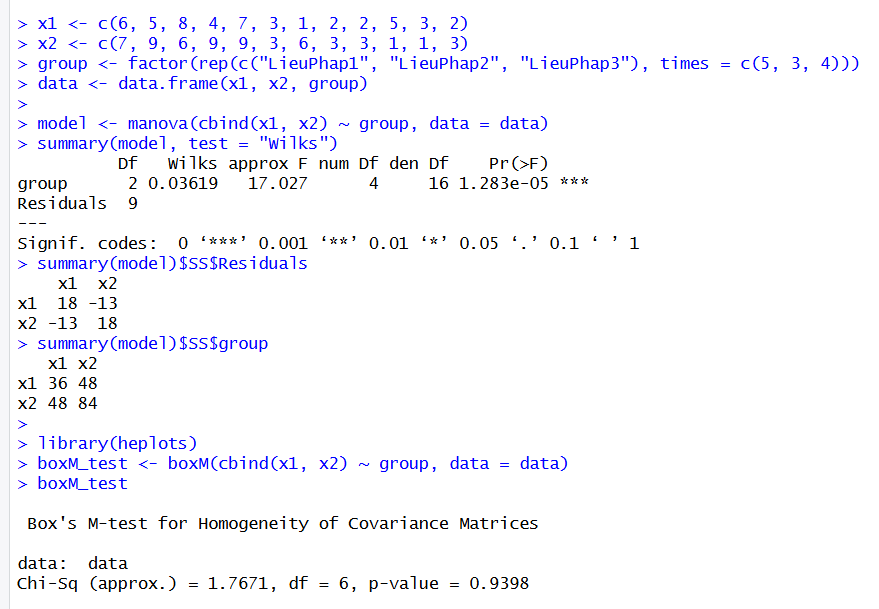
\includegraphics[width=0.9\textwidth]{ketqua4b.png}
    \caption{Kết quả chạy R: MANOVA và Box's M test}
\end{figure}

\textbf{3. Nhận xét và Kết luận}

Dựa vào các kết quả trích xuất từ phần mềm R (như ảnh trên), ta rút ra các nhận xét sau:

\begin{itemize}
    \item \textbf{Đối chiếu Ma trận W, B và Wilks' Lambda:} 
    Kết quả xuất ra từ hàm \texttt{summary(model)\$SS} cho ma trận Residuals ($W$) và ma trận Group ($B$) \textbf{hoàn toàn khớp với kết quả tính tay} ở câu A. Giá trị Wilks' Lambda từ phần mềm trả về chính xác là \textbf{0.03619}, cũng khớp với tính toán lý thuyết.
    
    \item \textbf{Kiểm định Box's M (Đồng nhất ma trận hiệp phương sai):}
    \begin{itemize}
        \item \textit{Giả thuyết $H_0$:} Ma trận hiệp phương sai của các nhóm là đồng nhất ($\Sigma_1 = \Sigma_2 = \Sigma_3$).
        \item \textit{Kết luận:} Giá trị \texttt{p-value = 0.9398} của kiểm định Box's M lớn hơn rất nhiều so với mức ý nghĩa $\alpha = 0.05$. Do đó, ta \textbf{chưa đủ cơ sở để bác bỏ $H_0$}. Điều này khẳng định dữ liệu hoàn toàn thỏa mãn giả định đồng nhất ma trận hiệp phương sai, cho phép kết quả của mô hình MANOVA là đáng tin cậy.
    \end{itemize}
    
    \item \textbf{Kiểm định MANOVA (Sự khác biệt giữa các nhóm):}
    \begin{itemize}
        \item Dựa vào kết quả của hàm \texttt{summary(model, test="Wilks")}, giá trị \texttt{p-value} (Pr(>F)) của thống kê Wilks' Lambda là \textbf{$1.283 \times 10^{-5}$}.
        \item Vì \texttt{p-value < 0.01}, ta \textbf{bác bỏ giả thuyết $H_0$} về sự bằng nhau của các vector trung bình.
        \item \textit{Kết luận chung:} Có sự khác biệt rất rõ rệt và mang ý nghĩa thống kê về hiệu quả của 3 liệu pháp lên hai biến đáp ứng $x_1$ và $x_2$.
    \end{itemize}
\end{itemize}

\section*{BÀI 5: Phân tích thành phần chính (PCA)}

\textbf{1. Nên giữ lại mấy thành phần chính? Vì sao?}
\\
Ta nên giữ lại \textbf{4 thành phần chính}.
\begin{itemize}
    \item \textbf{Giải thích:} Theo tiêu chuẩn Kaiser (Kaiser's Rule), ta chỉ giữ lại các thành phần chính có Eigenvalue lớn hơn 1 (đối với dữ liệu đã chuẩn hóa). Dựa vào Bảng 1, các Eigenvalue của 4 PC đầu lần lượt là 4.588, 2.119, 1.320, 1.195 đều $> 1$. PC5 có Eigenvalue là $0.468 < 1$ nên loại. Đồng thời, 4 PC này giải thích được \textbf{92.24\%} tổng phương sai của dữ liệu, một tỷ lệ rất cao và đủ tốt để giữ lại thông tin.
\end{itemize}

\textbf{2. Liệt kê các thành phần chính được chọn:} 
\\
Các thành phần chính được chọn là: \textbf{PC1, PC2, PC3, PC4}.

\textbf{3. Các biến góp phần lớn xây dựng hai thành phần đầu tiên (PC1, PC2) và giải thích?}
\\
Dữ liệu đề bài cung cấp là ma trận Rotation từ lệnh \texttt{prcomp()} trong R, tức các giá trị là \textbf{Vector riêng} ($e_{ik}$), với tổng bình phương mỗi cột bằng 1. Để xác định mức độ đóng góp của từng biến, ta dùng giá trị tuyệt đối của $e_{ik}$ để so sánh tương đối (biến nào có $|e_{ik}|$ lớn hơn thì đóng góp nhiều hơn vào TPC đó). Nếu muốn tính hệ số tương quan chính xác, cần nhân thêm $\sqrt{\lambda_i}$.

\begin{itemize}
    \item \textbf{Đối với PC1 (giải thích 45.88\% phương sai):}
    \begin{itemize}
        \item \textbf{Hệ số dương lớn:} MENA (0.420), ENFA (0.407).
        \item \textbf{Hệ số âm lớn:} TRAN (-0.457), PROF (-0.456).
        \item \textit{Ý nghĩa:} PC1 phân định rõ sự tương phản giữa quỹ thời gian dành cho \textbf{"Gia đình/Việc nhà"} (Dọn dẹp, Con cái) mang giá trị dương, với \textbf{"Công việc xã hội"} (Đi lại, Nghề nghiệp) mang giá trị âm. Đây là thành phần đại diện cho cán cân giữa công việc ngoài xã hội và việc gia đình.
    \end{itemize}
    \item \textbf{Đối với PC2 (giải thích 21.19\% phương sai):}
    \begin{itemize}
        \item \textbf{Hệ số dương lớn:} REPA (0.459), SOMM (0.391).
        \item \textbf{Hệ số âm lớn:} TOIL (-0.561), COUR (-0.522).
        \item \textit{Ý nghĩa:} PC2 đại diện cho sự đối lập giữa quỹ thời gian dành cho \textbf{"Nhu cầu nghỉ ngơi sinh lý cơ bản"} (Ăn uống, Ngủ) mang giá trị dương và các hoạt động \textbf{"Sinh hoạt cá nhân/Mua sắm ngoài"} (Vệ sinh, Đi chợ) mang giá trị âm. Trục này đi sâu vào việc phân tách các thói quen chăm sóc cá nhân.
    \end{itemize}
\end{itemize}

\end{document}